\documentclass[10pt,a4paper]{report}
\usepackage[utf8]{inputenc}
\usepackage{amsmath}
\usepackage{amsfonts}
\usepackage{amssymb}

\usepackage{fullpage}
\usepackage{url}
\usepackage[numbers,square]{natbib}
\AtBeginDocument{\renewcommand{\bibname}{References}}

\author{Jacek Czyrnek, Adam Koleszar, Marion Le Guével, Mihaly Lengyel
•
}
\usepackage{graphicx}
\usepackage{indentfirst}
\title{Group project report}

\begin{document}
\maketitle
\tableofcontents

\chapter{Introduction}
Optimisation process is a big part in the domain of engineering. It applies for a very wide amount of subjects, and for many, it can be a very heavy and long treatment requiering a lot of ressources. That is because of these costs, that a monitoring and recovering system is always needed if any problem could happen during the optimisation process. That way, not all the treatment is lost, and it is not necessary to restart it from the beginning.\\

This project report is dealing with the purpose of its realization in Chapter 1. Then, the previous researches done to define a good recovery system are presented in Chapter 2. Chapter 3 explains what the project needs to provide and Chapter 4 the choices about how to provide it. Finally, Chapter 5 shows what the project actually looks like, Chapter 6 how the testing phase where handled and Chapter 7 what problems where encountered by the team, to end with a conclusion in Chapter 8.\\

The aim of the project itself, is to design and developp a distributed system for monitoring the progress of the aerofoil design optimisation through an intuitive user interface with a login access. The main point is not the optimisation but the recovery system behind it.

As students working in engineering, the objective is to test all the skills needed to do a project. Indeed, it's not only about working in the subject of optimisation or doing an actual monitoring and recovery system, but also working as a team. This means planning and organizing the tasks to design and code the project with a good communication, and finishing with a presentation of what has been done.

\chapter{Technical review}
All computer systems are composed of many subsystems which can encounter problem or failure preventing them to do their tasks. Because of this, those systems can stop working and, then, loose all their data and progression.

That's why every reliable and secure system takes into account the risk of sudden failure of any of its component. Most of the time, it includes communication between those components and action depending on the analysis of the failure. However, the monitoring and recovery plan is different for each system as each system as its own design and components. Therefore many approaches has been implemented to handle different events of numerous examples of systems. 

	\section{Automatic action}
		\subsection{Cluster environment}
Cluster systems are complex in a way that it is a distributed environment. This means that there are a lot of independent components communicating together for one common result. Failures can, then, appear on many places. 

A way to locate an error is through a heartbeat protocole [1][2] which makes each component send a signal at regular intervals to another one. As soon as the error has been detected, there are different options. 
Some recovery softwares already exist, but there are very expensive and it requiers to install it on every node, paying for each of them [1].
You can have a recovery driver which will analyze and execute recovery actions [1]. If it fails, it will complete the remaining actions anyway. 
There is also a possibility to use a spare server to take over the job. If the heartbeat signal stops, the spare server will do the job instead of the one crashed. However, it means that there is a server inactive most of the time, waiting for a failure, which is a waste of money. This is why Dias [2] proposes to use a spare server which is actually working with the others even when there is no failure.

		\subsection{Software environment}
Software environment can be on a server or on a local machine. It is quite a large form which includes different type of faults. Delgado [3] exposes the classification of the software fault monitoring system. She explains the use of graphs to detect the violation and call the good function in Java depending of the fault to, finally, enforced the synchronization. To evaluate the error, some measures can be used like tasks performance or other metrics [4]. A pre-compiler can also be used to correct errors automatically [5] or a "self-healing" method which reverse faulty until failure is avoided [6].
		
	\section{User action}	
Many errors can be easily detected during the execution of the system, and, then, automatically handled with pre-determined solutions (see previous section). For other types of errors, it requiers the intervention of a human being. 

In a computing environment, a hot key can be selected by the end user at pre-boot or runtime phase to perform a precise recovery action [7]. This solution is limited by the technical level of the end user as well as the configuration of the computer. 

In a database, once a wrong request has been executed most of the time the only solution is to restore the full database. All the wrong actions are, then, deleted, but also some good ones. Thus, the consistency is lost. Zwilling [8] suggests to regularly create some snapshots of the change in the database (and not all of it) and some more on specific events. That way, a human being can just go back through some snapshots and find the one that shouldn't be executed without loosing all the other changes.

	\section{Previous researches and current project}
The current project uses an educational Java code from NASA modified to correspond to the current system. This part of the execution is runned on a cluster (see Implementation Chapter) but there is no possibility to manage it. That is why handle possible errors can't be done at the infrastructure level. The solution of the logs on the server is the best in this case to track the error and recover from it. 

The main part of the software is on local machine. Therefore, all the results are stored in a local database file. If an error appears in the database, the logs can also restore it.



\chapter{Requirements specifications}
	\section{Usecases}
This project handle login as sessions. Therefore each session (a set of iterations) is a new user with a new password.  However, all these "users" are of the same type and have the same functionnalities : \\
\begin{figure}[h!]
\includegraphics[scale=0.7]{Usecase_group-project.png}\\
\caption{Usecase}
\end{figure}


Mainly, the purpose of this software is to solve an equation with different given parameters and to display the result graphically.
	\section{Functional and non functional requirements}
On the previous usecase, different functionalities are written. This subsection will detailed those functionalities into functional and non functional requirements.
		\subsection{Functional requirements}
\begin{tabular}{|c|c|}
\hline 
\textbf{ID} & \textbf{Requirement} \\ 
\hline 
1 & To log into a session \\ 
\hline 
2 & To create a new session \\ 
\hline 
3 & As logged in : To enter new inputs \\ 
\hline
4 & As logged in : To start or stop iterating on the equation (exchange of data with the cluster) \\ 
\hline
5 & As logged in : To display the result of the iterations in real time on a graph \\ 
\hline
6 & As logged in : To display the result of the iterations in real time as a wing modeling \\ 
\hline
7 & As logged in : To download the log file (exchange of data with the cluster)\\ 
\hline
8 & As logged in : To logout from a session \\ 
\hline
\end{tabular} 
		\subsection{Non-functional requirements}
\begin{tabular}{|c|c|}
\hline 
\textbf{Type} & \textbf{Requirement} \\ 
\hline 
Security & To log into a session with a password so only people having those\\
 & information can access to it\\ 
\hline 
Reliability & To have a recovery system to access previous steps of a session \\ 
\hline 
Speed & To use a cluster for solving the equation \\ 
\hline
\end{tabular} 
	\section{Further information}
An example has been given for the software user interface. With the functionalities required, the final product should have two "pages", one for the connexion or creation of a session, and another one once logged in a session, as the mockups below:\\
\begin{figure}[h!]
\includegraphics[scale=0.5]{group_project_mockups.png}
\caption{Mockup}
\end{figure}


\pagebreak
\chapter{System design}
\section{Component diagram}
We began the design process by dividing the system into bigger modules and designing the interfaces between them to conduce parallel work. We split the software into 4 bigger modules and assigned one to each team member:\\
\begin{enumerate}
\item Database \& Session: Marion Le Guével
\item Atlas Connector: Ádám Koleszár
\item GUI: Jacek Czyrnek
\item Wing Visualizer: Mihály Lengyel
\end{enumerate}
The following diagram shows the components of the system and the interfaces they interact through.
\begin{figure}[h!]
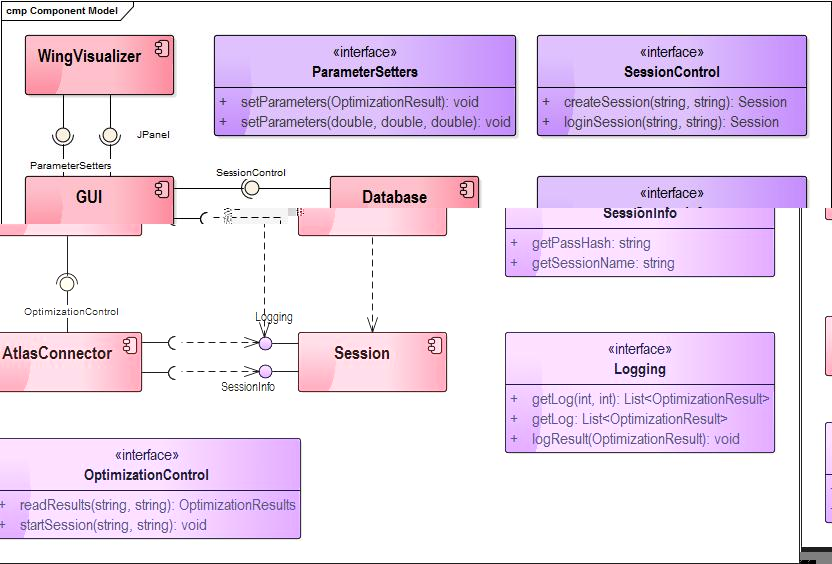
\includegraphics[width=\textwidth]{CompModel.jpg}
\caption{Component diagram}
\end{figure}
\pagebreak

\section{Class diagram}
In the following diagram you can see, that the classes in the implemented system are simple reflections of the component design above.
\begin{figure}[h!]
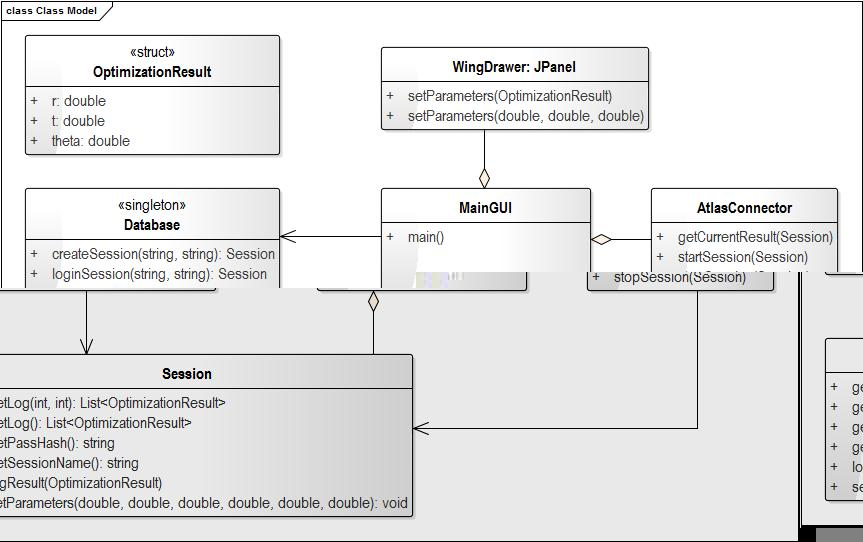
\includegraphics[width=\textwidth]{ClassModel.jpg}
\caption{Class diagram}
\end{figure}
\pagebreak
\section{Sequence diagram}
To complement the static diagrams above here we provide a diagram to show the dynamic behaviour of the system. This is not an exact sequence diagram but it shows the flow of data through the system.
\begin{figure}[h!]
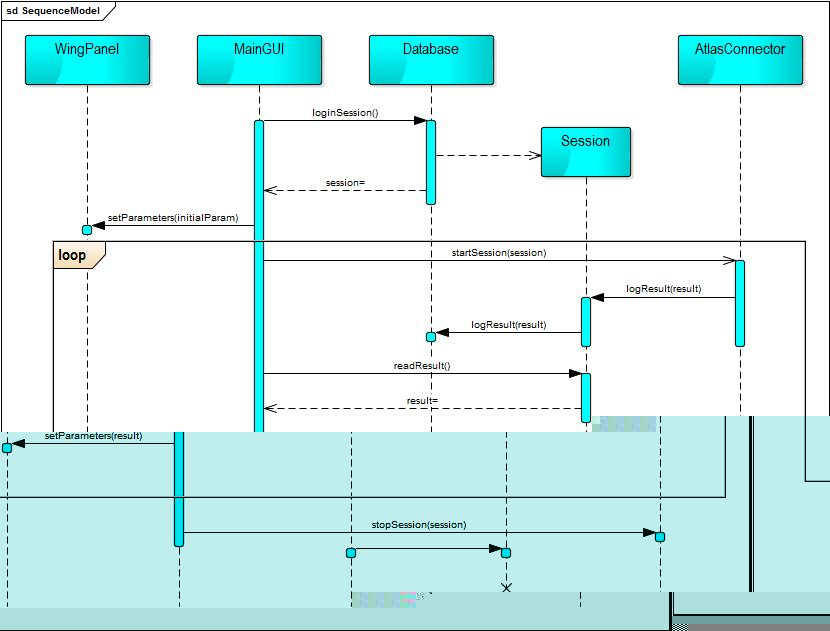
\includegraphics[width=\textwidth]{SequenceModel.jpg}
\caption{Sequence diagram}
\end{figure}

\chapter{Implementation}
\subsection{Database}
We used the SQLite single file database solution as our database, and for it to work with our JAVA application we used the open-source SQLite JDBC driver \cite{WWW:SQLite}.

\subsection{Cluster connection}
As a cluster we used the power of the Astral \footnote{10240 nodes} university cluster, which can be reached via SSH protocol. In order to connect to the servers from our software we used the open-source JSch package from JCraft \cite{WWW:JSCH}. It allowed us the connect to the gate server, copy our solver on it via SCP (secured copy) and start the computation. The result are also coming back on the SSH connection as remote command execution.

For user authentication we created our own handler which uses the interfaces provided by the JSch package. It handles the password prompt and other connection configuration as well silently, so the user only need to type in his or her username and password.

\subsection{Remote computation}
Although our software contains the solver component as well, due Java version differences on the Astral server we decided to create a separate software that handles the computation and can run on the remote machines.

It is a command line application. It has several parameter options. To handle these command line parameters we used the open-source CLI commons package from Apache \cite{WWW:CLI}.

\subsubsection{Solver}
It is based on the previously mentioned NASA air foil simulation educational JAVA applet \cite{WWW:NASA}. Because it contained computation for several other environment that is different for the normal Earth conditions we removed most irrelevant parts from it. The solver now can compute dimensionless lift and drag forces for given wing geometrics.

\subsubsection{Optimizer}
The optimizer is also part of the remote program. It takes parameter intervals for the wing geometrics and optimizes the lift drag ratio between those intervals returning the optimized wing geometrics. It also logs whenever a better solution is found.

\chapter{Failure case studies}
In this chapter we are going to write about the various failures that can occur during execution of the program and the way they can be avoided or repaired.

\section{Communication errors}
For a system that uses external connections to transfer data between components (like a network) is bound to have some communication errors in time. These can be disconnection issues, data corruption, security issues. As programmers we have to ensure that the system will properly handle these issues without too much data loss.

Failure to do so will lead to the waste of significant computation effort, which can be ultimately translated to the loss of money and time. To avoid or to be prepared for these cases the following measures were taken.

\subsection{Disconnection}
If a network connection disconnects it is only allowed to lose the data being sent, nothing more. For this, proper and thorough logging system needs to be implemented. In our case it is client and server side logging as well.

\subsection{Server side logging}
On the server side simple log files are created. Every line contains the best solution at that point in time. The solution contains the angle of attack, the camber size relative to the chord and the thickness of the wing relative to the chord. The solution also contains the computed the dimensionless values of the lift and drag forces and the ratio of the two for easier data readability. The help the finding of data on the server the log files are named after the session name.

\subsection{Client side logging}
The sessions and the computed values are also logged on the client side of the application. These data are stored in the SQLite database file attached to the program. From that any computation session and it's result can be restored and even continued if the computation didn't finish.

\subsection{Transfer error}
If the messages between the server and the client side get corrupted for any kind of reason, the messages will get discarded, and user will get a notification about possible communication error. The computation will continue and produce relevant data on the server side. If the data in between is not relevant the results can be gathered from the server log, if they are relevant as well, the computation can continue from the last correct message.

\subsection{SSH related errors}
Before the computation could start the program needs to copy the computing part of the program to the remote machine. During these communications errors can occur either with the connection itself, or with the SSH protocol. Later errors include SSH server downtime, user authentication errors etc. Dealing with these issues is outside of the scope of our program, although the program will do anything so that no data should get lost. The program will notify the users about SSH errors, and computation won't start until such issues are handled.

\section{Database error}


\section{Software error}
\subsection{Server side error}
\subsection{Client side error}

\chapter{Conclusion}
This group project was a good exercise to make us use all the knowledge we gathered throughout the last semester, and provided a quick introduction into making a complete product through teamwork.

We used JAVA programming language and technologies to implement our solution.
\begin{flushleft}
	\bibliographystyle{newapa}
	\bibliography{bibliography}
	\addcontentsline{toc}{chapter}{References}
\end{flushleft}


\end{document}